\chapter{Design and Implementation}

(approx. 10 pages)\\

* Check if you have addressed Provided a graphical representation for your design?\\
* Provided a Project folders and files diagram?\\

\section{Program Design and Interaction Mechanisms} %TODO: Everybody, yeaahhhh ;)
* Approach to design\\
* important issues and choices and their relationships to theoretical concepts and the hardware and software platforms\\
* Did you use the GPIO module? How? In terms of interrupts and the setup in the main\\
* Did you use interrupts? How?\\ 
* Did you use multiple threads / handlers? How? Why?\\
* Did you use TI-RTOS? How?\\

\section{Main Functions and State Machine} %TODO: Hendrik

\begin{figure}[H]
	\begin{center}
		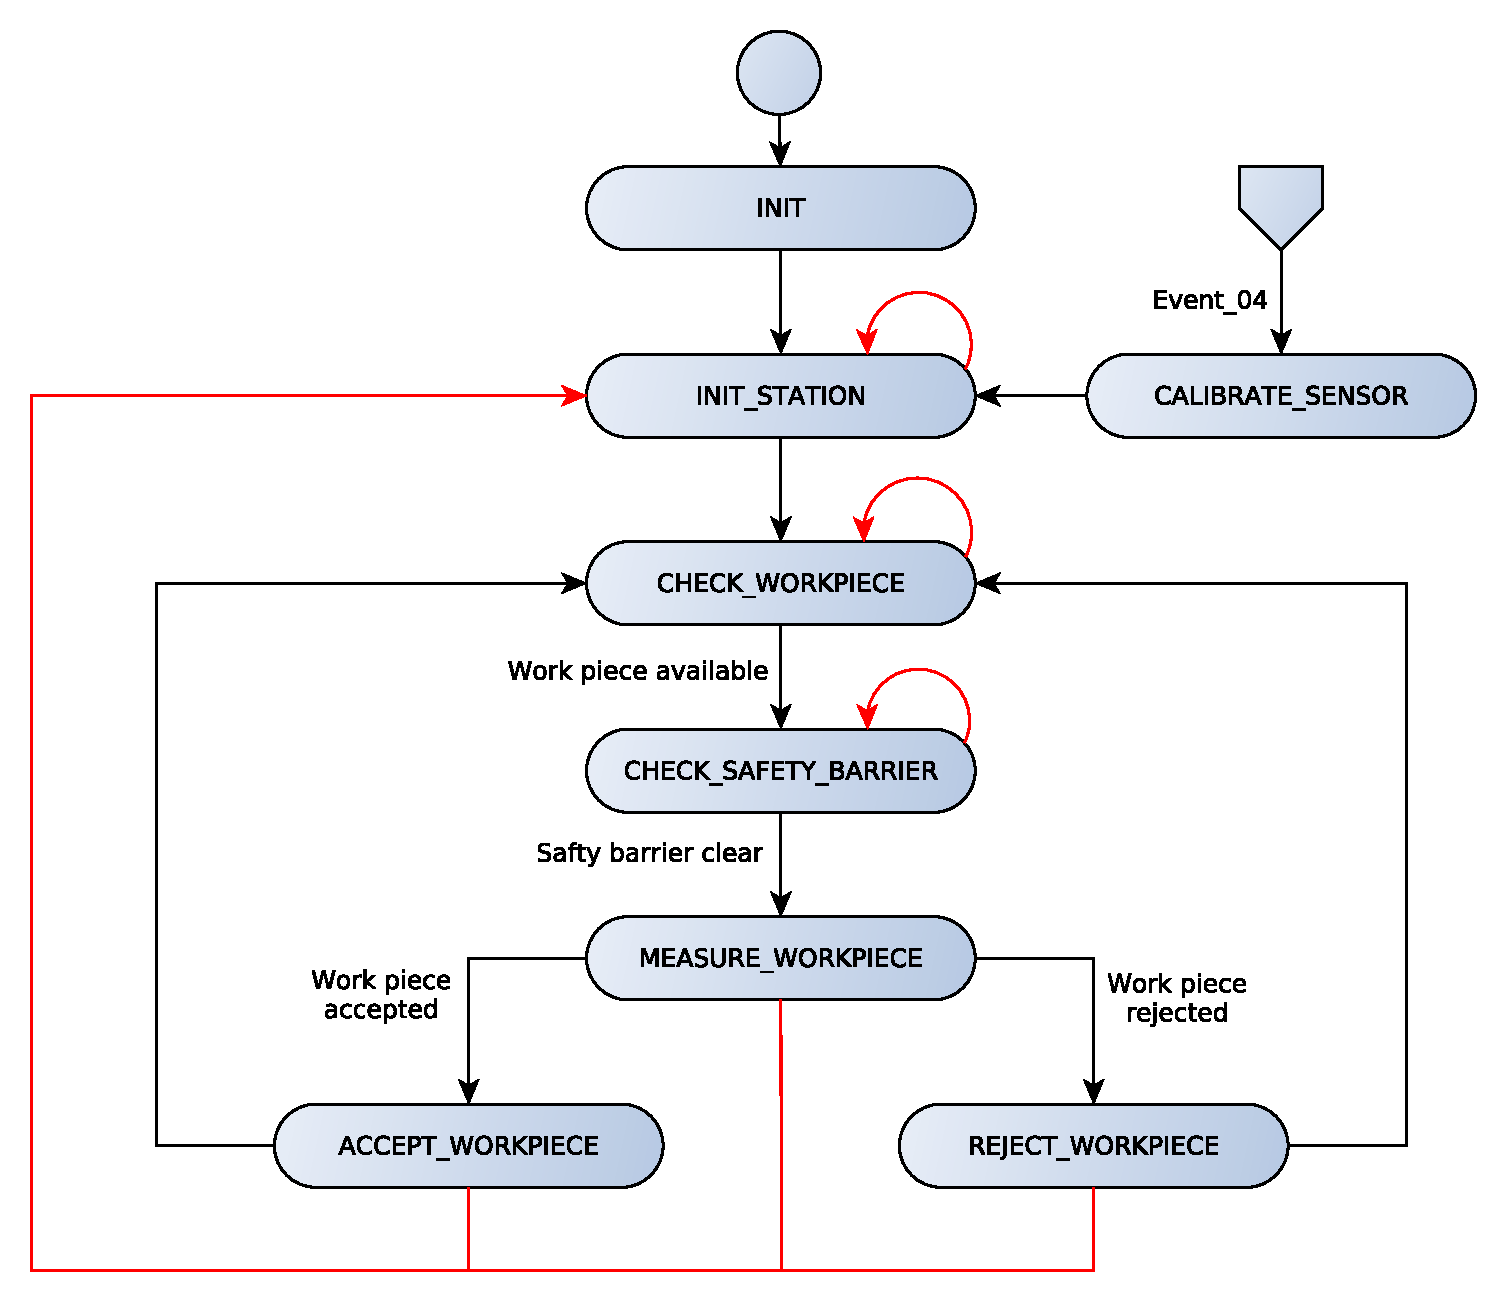
\includegraphics[scale=.60]{media/StateMachine_Main.pdf} 	
		\caption{Main State Machine}
		\label{fig:statemachine}
	\end{center}
\end{figure}

\section{Device Driver Library} %TODO: Timo
* Did you use the GPIO module? How? Through the qut library... Pin Map table?\\
* Did you use the ADC? How? 

% TODO: Table of measurements?

\begin{figure}[H]
	\begin{center}
		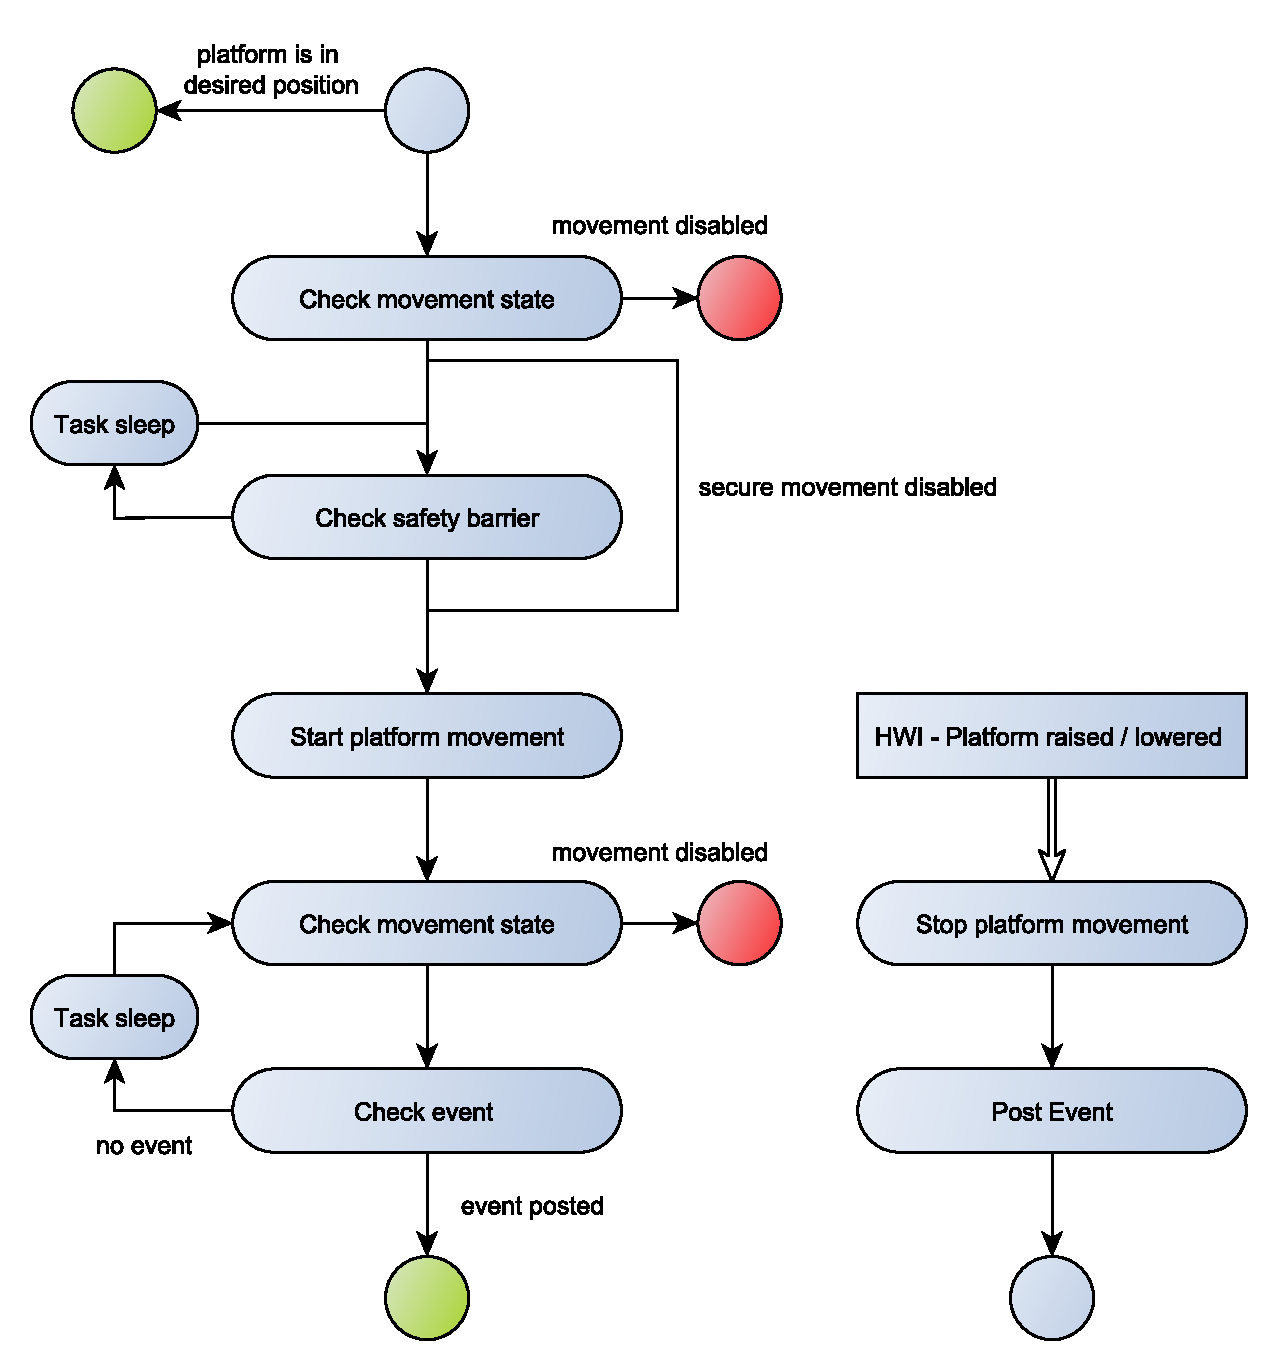
\includegraphics[scale=.60]{media/Flow_Chart_MovePlatform.pdf} 	
		\caption{Flow Chart Move Platform}
		\label{fig:moveplatform}
	\end{center}
\end{figure}

\section{User Interface} %TODO: Pixel-Julian
* Did you use the graphics library? How?\\



